% ═══════════════════════════════════════════════════════════════════
% ЧАСТЬ XII. АТЛАС ДИАГРАММ И КАТАЛОГ ФОРМУЛ
% ═══════════════════════════════════════════════════════════════════
\part{Атлас диаграмм и каталог формул}

\section{Атлас диаграмм}\label{sec:atlas}

Диаграммы настоящего атласа построены лабораторией в модульной
плиточной системе с разрешением $600$~dpi; каждая плитка
воспроизводится пунктом меню «Диаграммы» и сопровождается
комментарием, связывающим картинку с теоремами текста.

\begin{figure}[t]
\centering
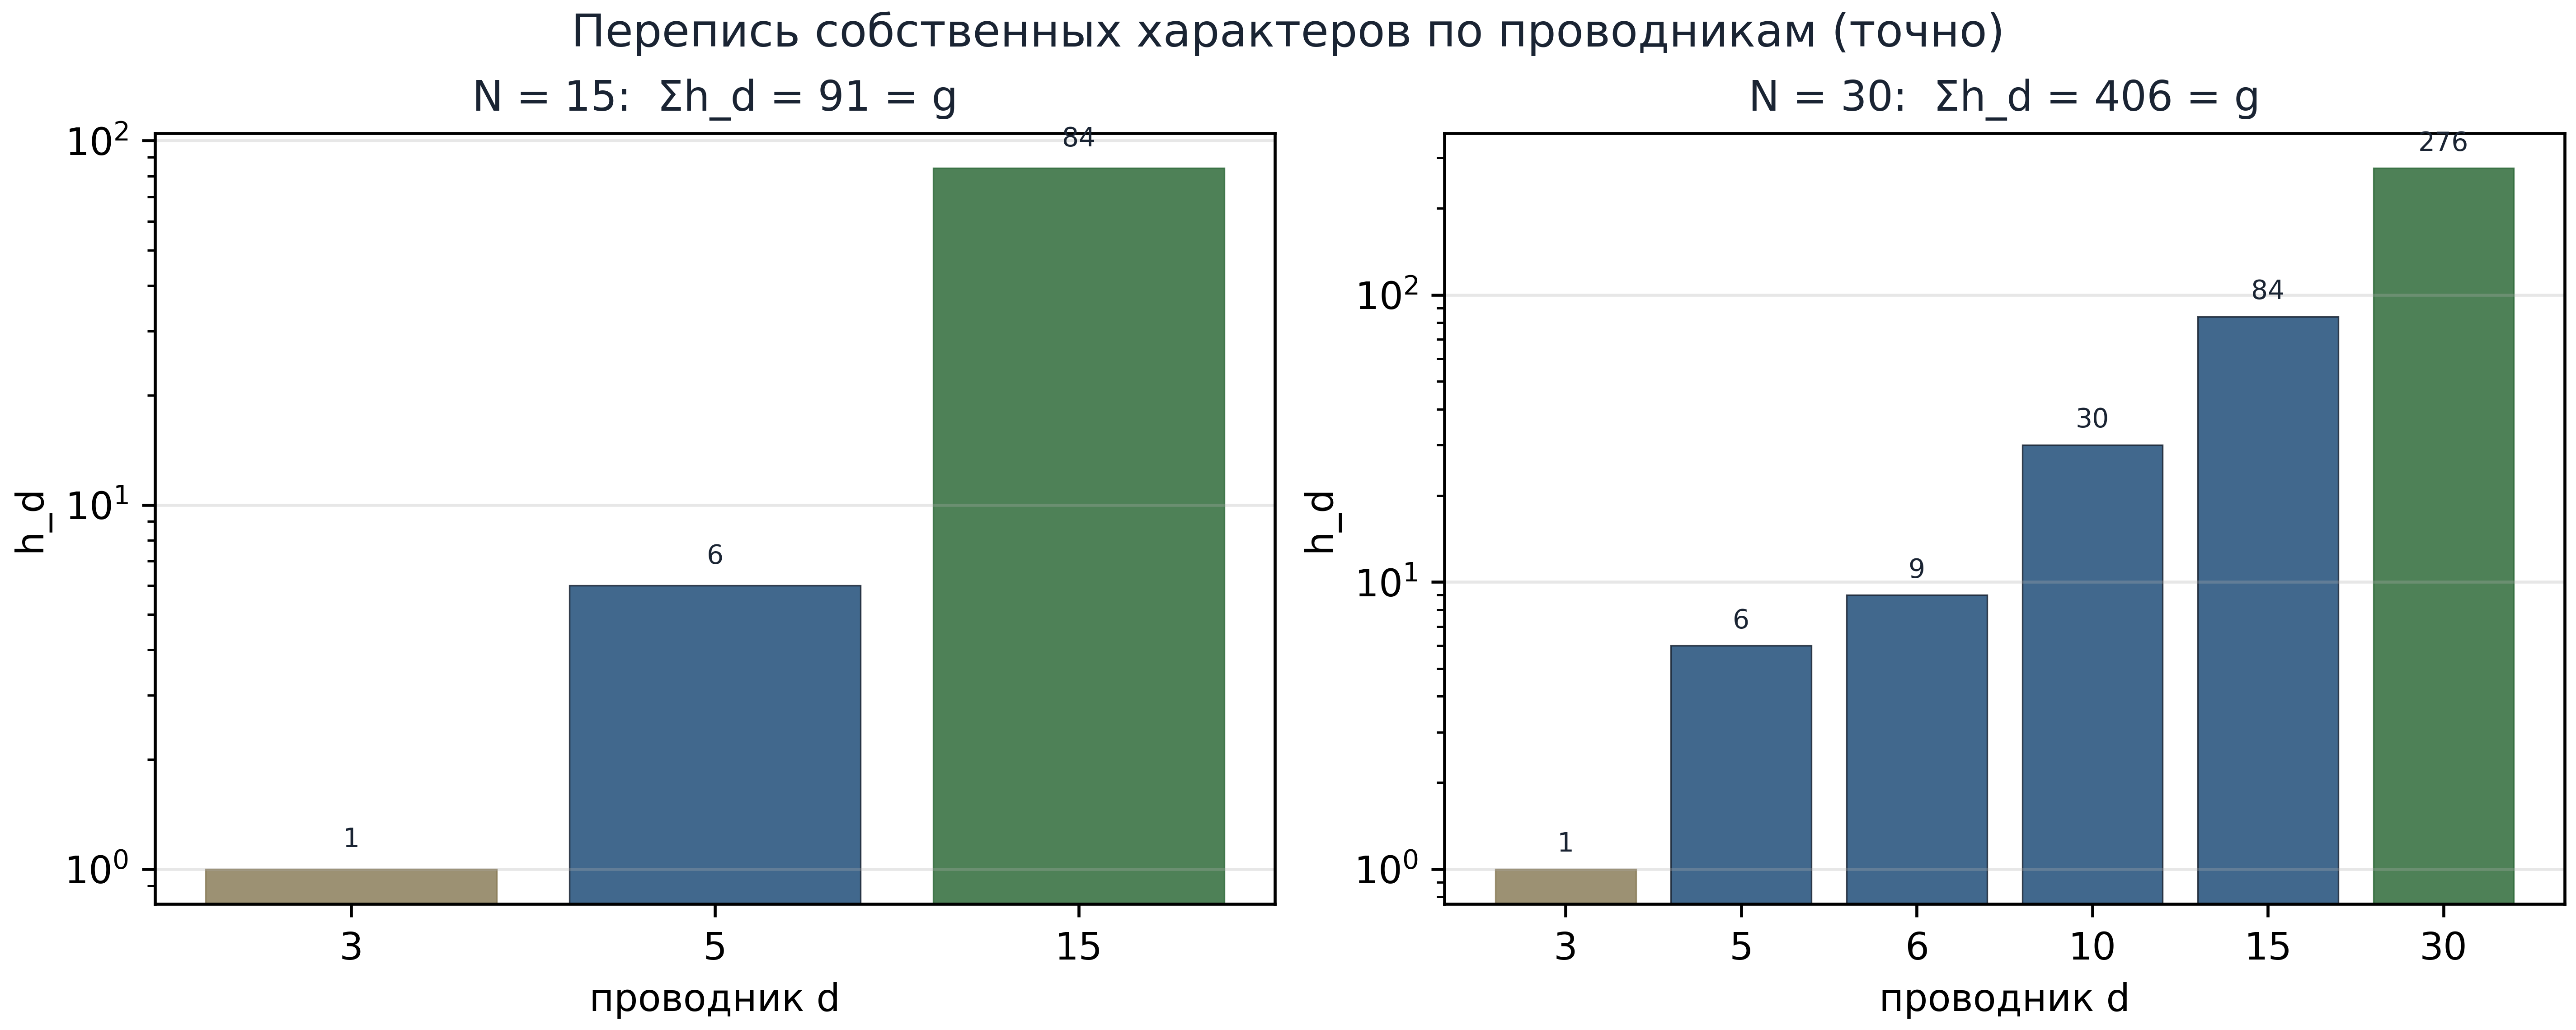
\includegraphics[width=\textwidth]{figs/fig_census.png}
\caption{Перепись собственных характеров по проводникам для
$N=15$ и $N=30$ (логарифмическая шкала). Высоты столбцов ---
точные целые $h_d$; суммы $1+6+84=91$ и
$1+6+9+30+84+276=406$ совпадают с родами
(лемма~\ref{lem:genus}, перепись~\eqref{eq:mobius}, проверка V1).
Выделены крайние блоки: тривиальные проводники $3$ (золотой) и
полный проводник (зелёный).}
\label{fig:census}
\end{figure}

\begin{figure}[t]
\centering
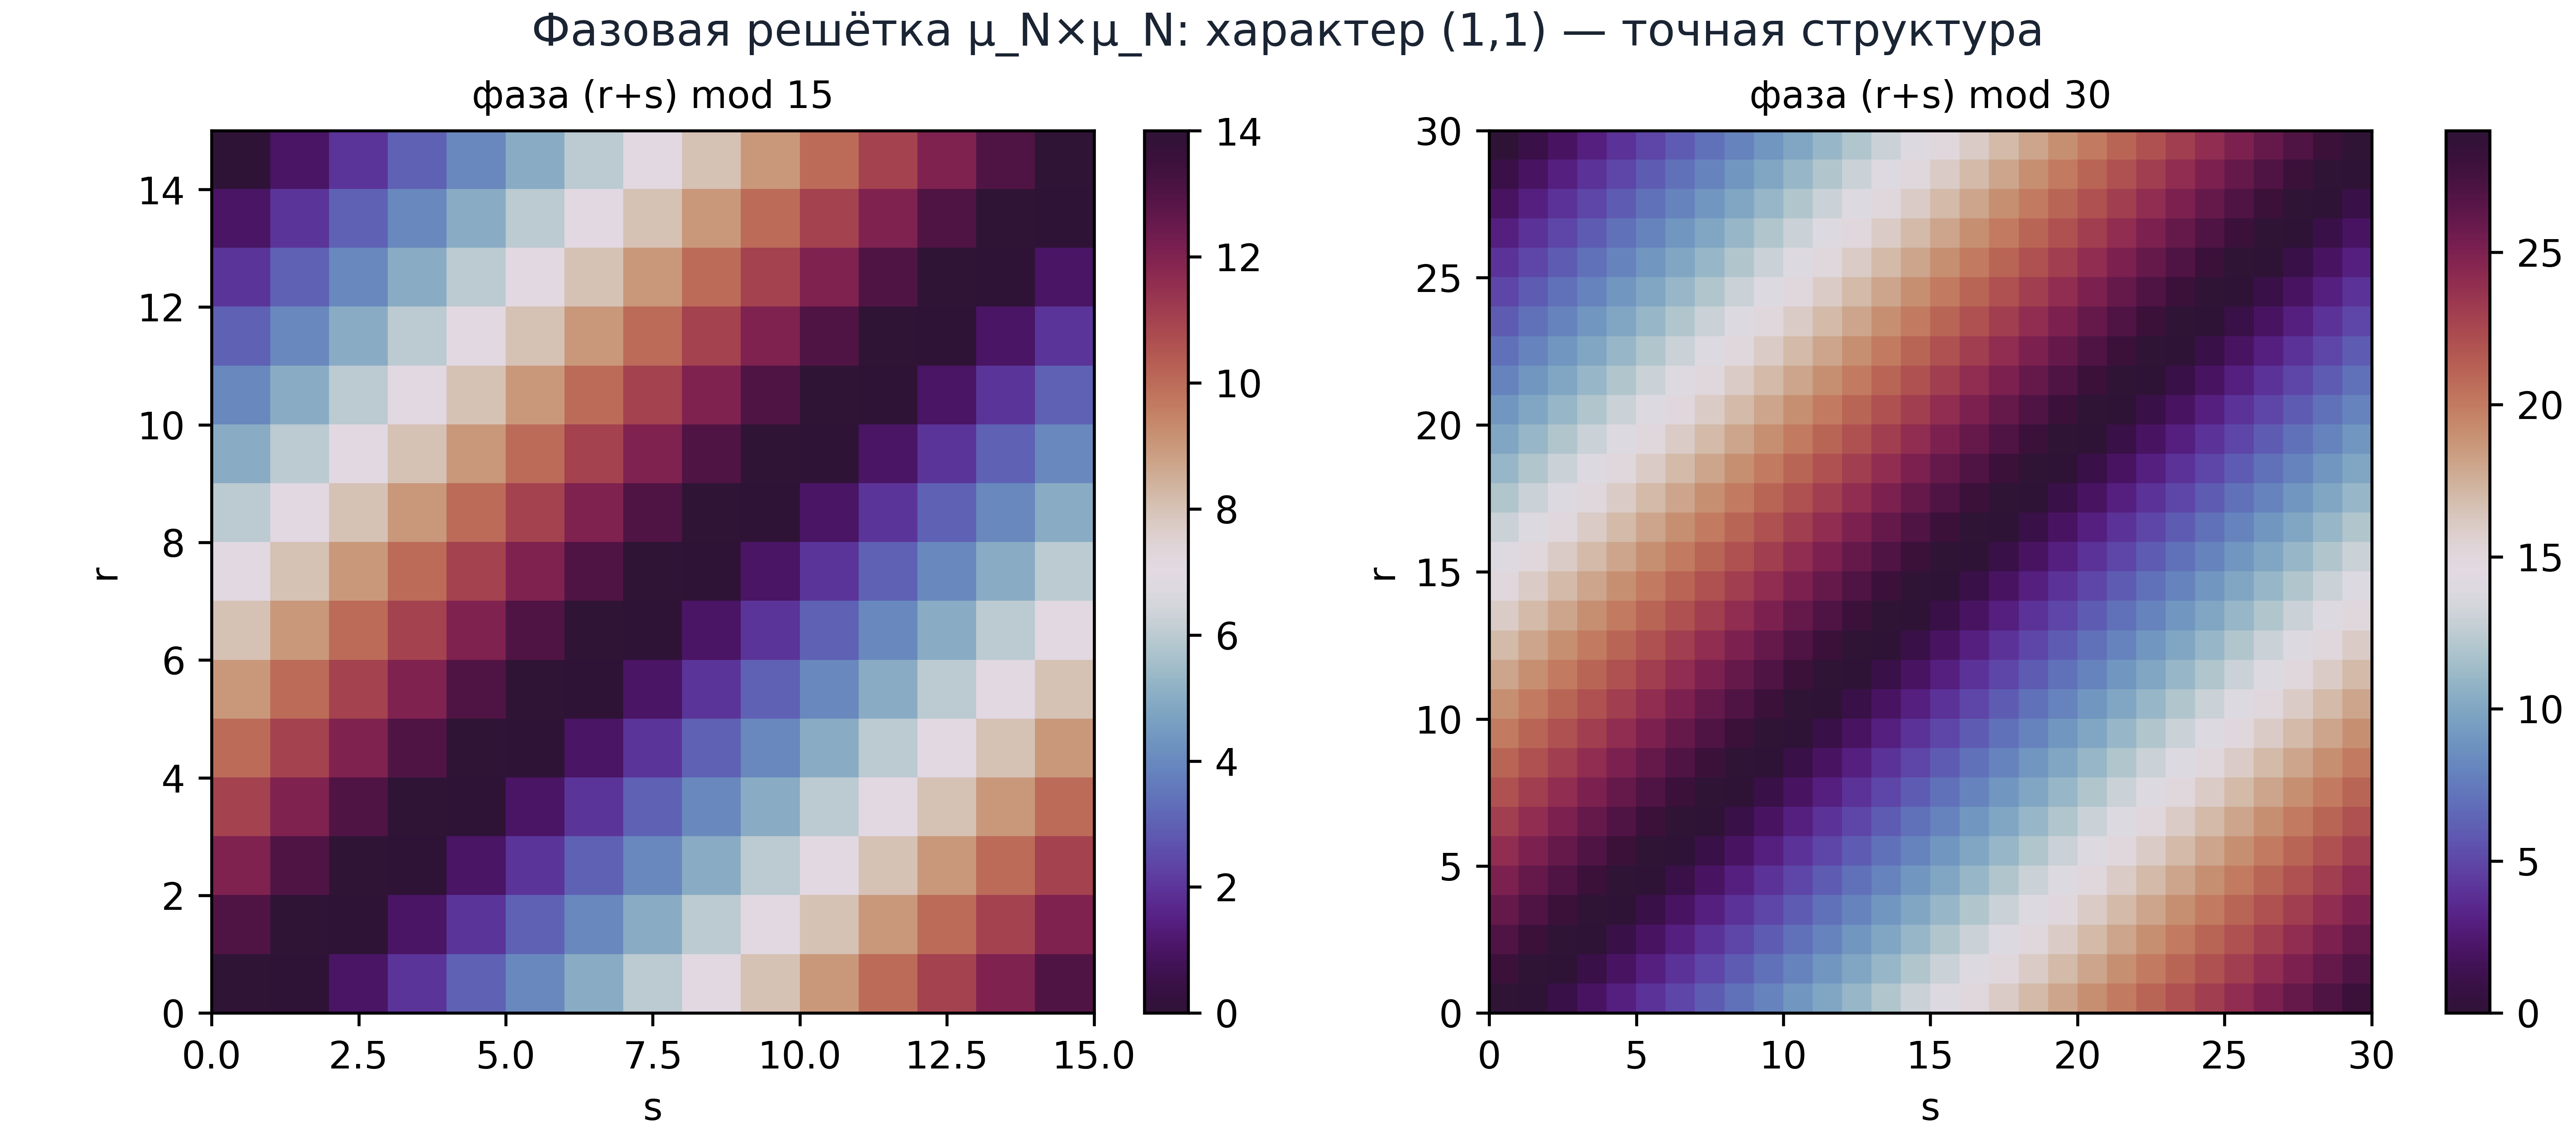
\includegraphics[width=\textwidth]{figs/fig_phasegrid.png}
\caption{Фазовая решётка $\mu_N\times\mu_N$: значения
$(r+s)\bmod N$ на торе $(\ZZ/N)^2$ для характера $(1,1)$.
Диагональные полосы --- в точности классы эквивалентности фазы
$\zeta_N^{ra+sb}$; точность фазы (V3: отклонение $0.0$) видна как
идеальная полосатость без разрывов.}
\label{fig:phasegrid}
\end{figure}

\begin{figure}[t]
\centering
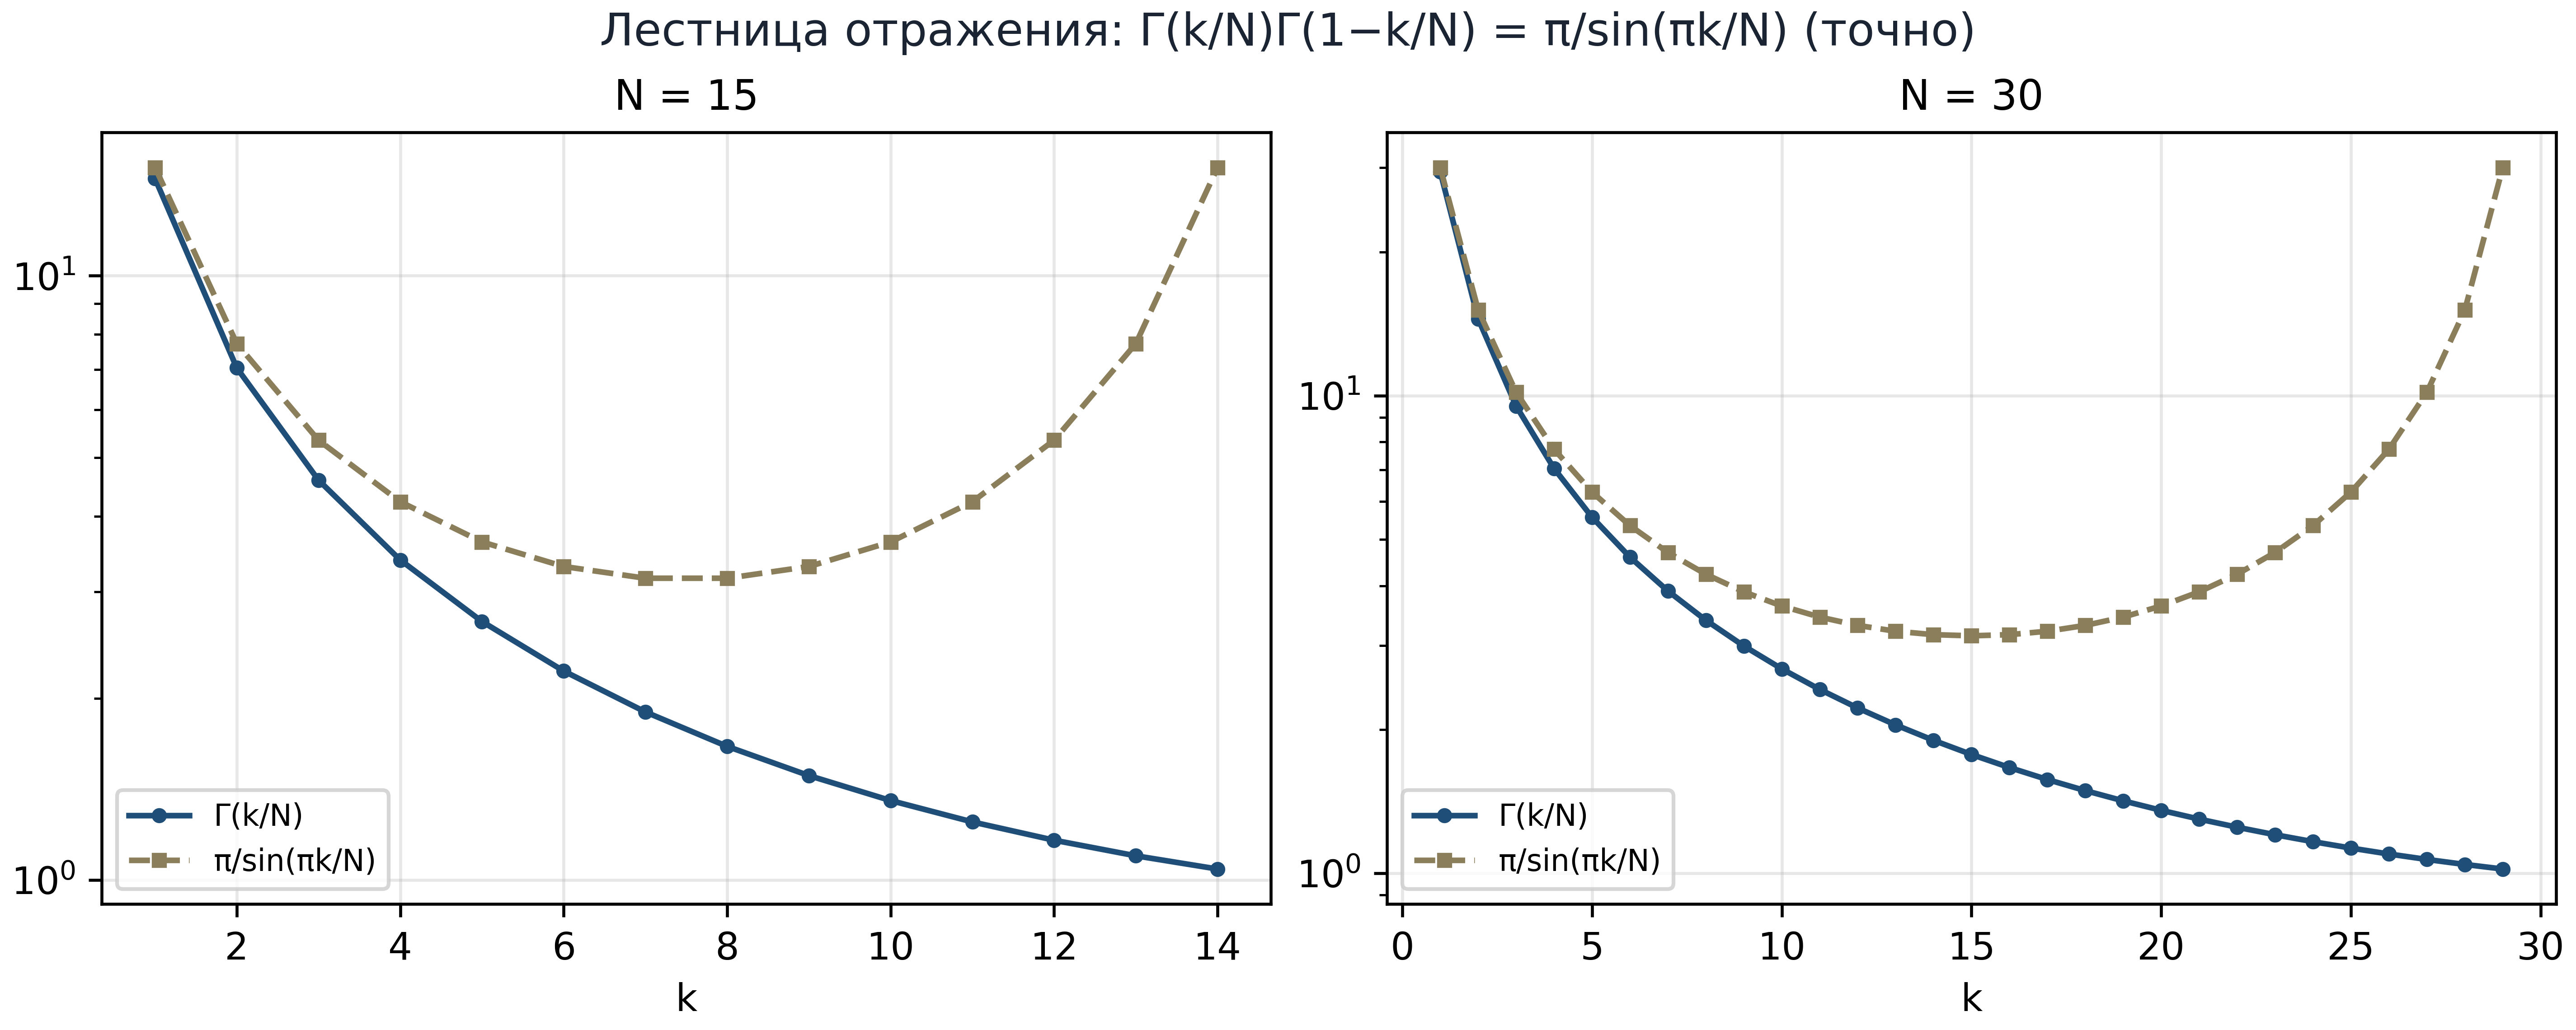
\includegraphics[width=\textwidth]{figs/fig_gamma.png}
\caption{Лестница отражения: $\Ga(k/N)$ против
$\pi/\sin(\pi k/N)$ (обе кривые в логарифмической шкале).
Совпадение кривых на обоих уровнях --- численный портрет
тождества леммы~\ref{lem:reflection}; максимальное отклонение по
всем $k$ составляет $7.0\cdot10^{-36}$ (проверка V6).}
\label{fig:gamma}
\end{figure}

\begin{figure}[t]
\centering
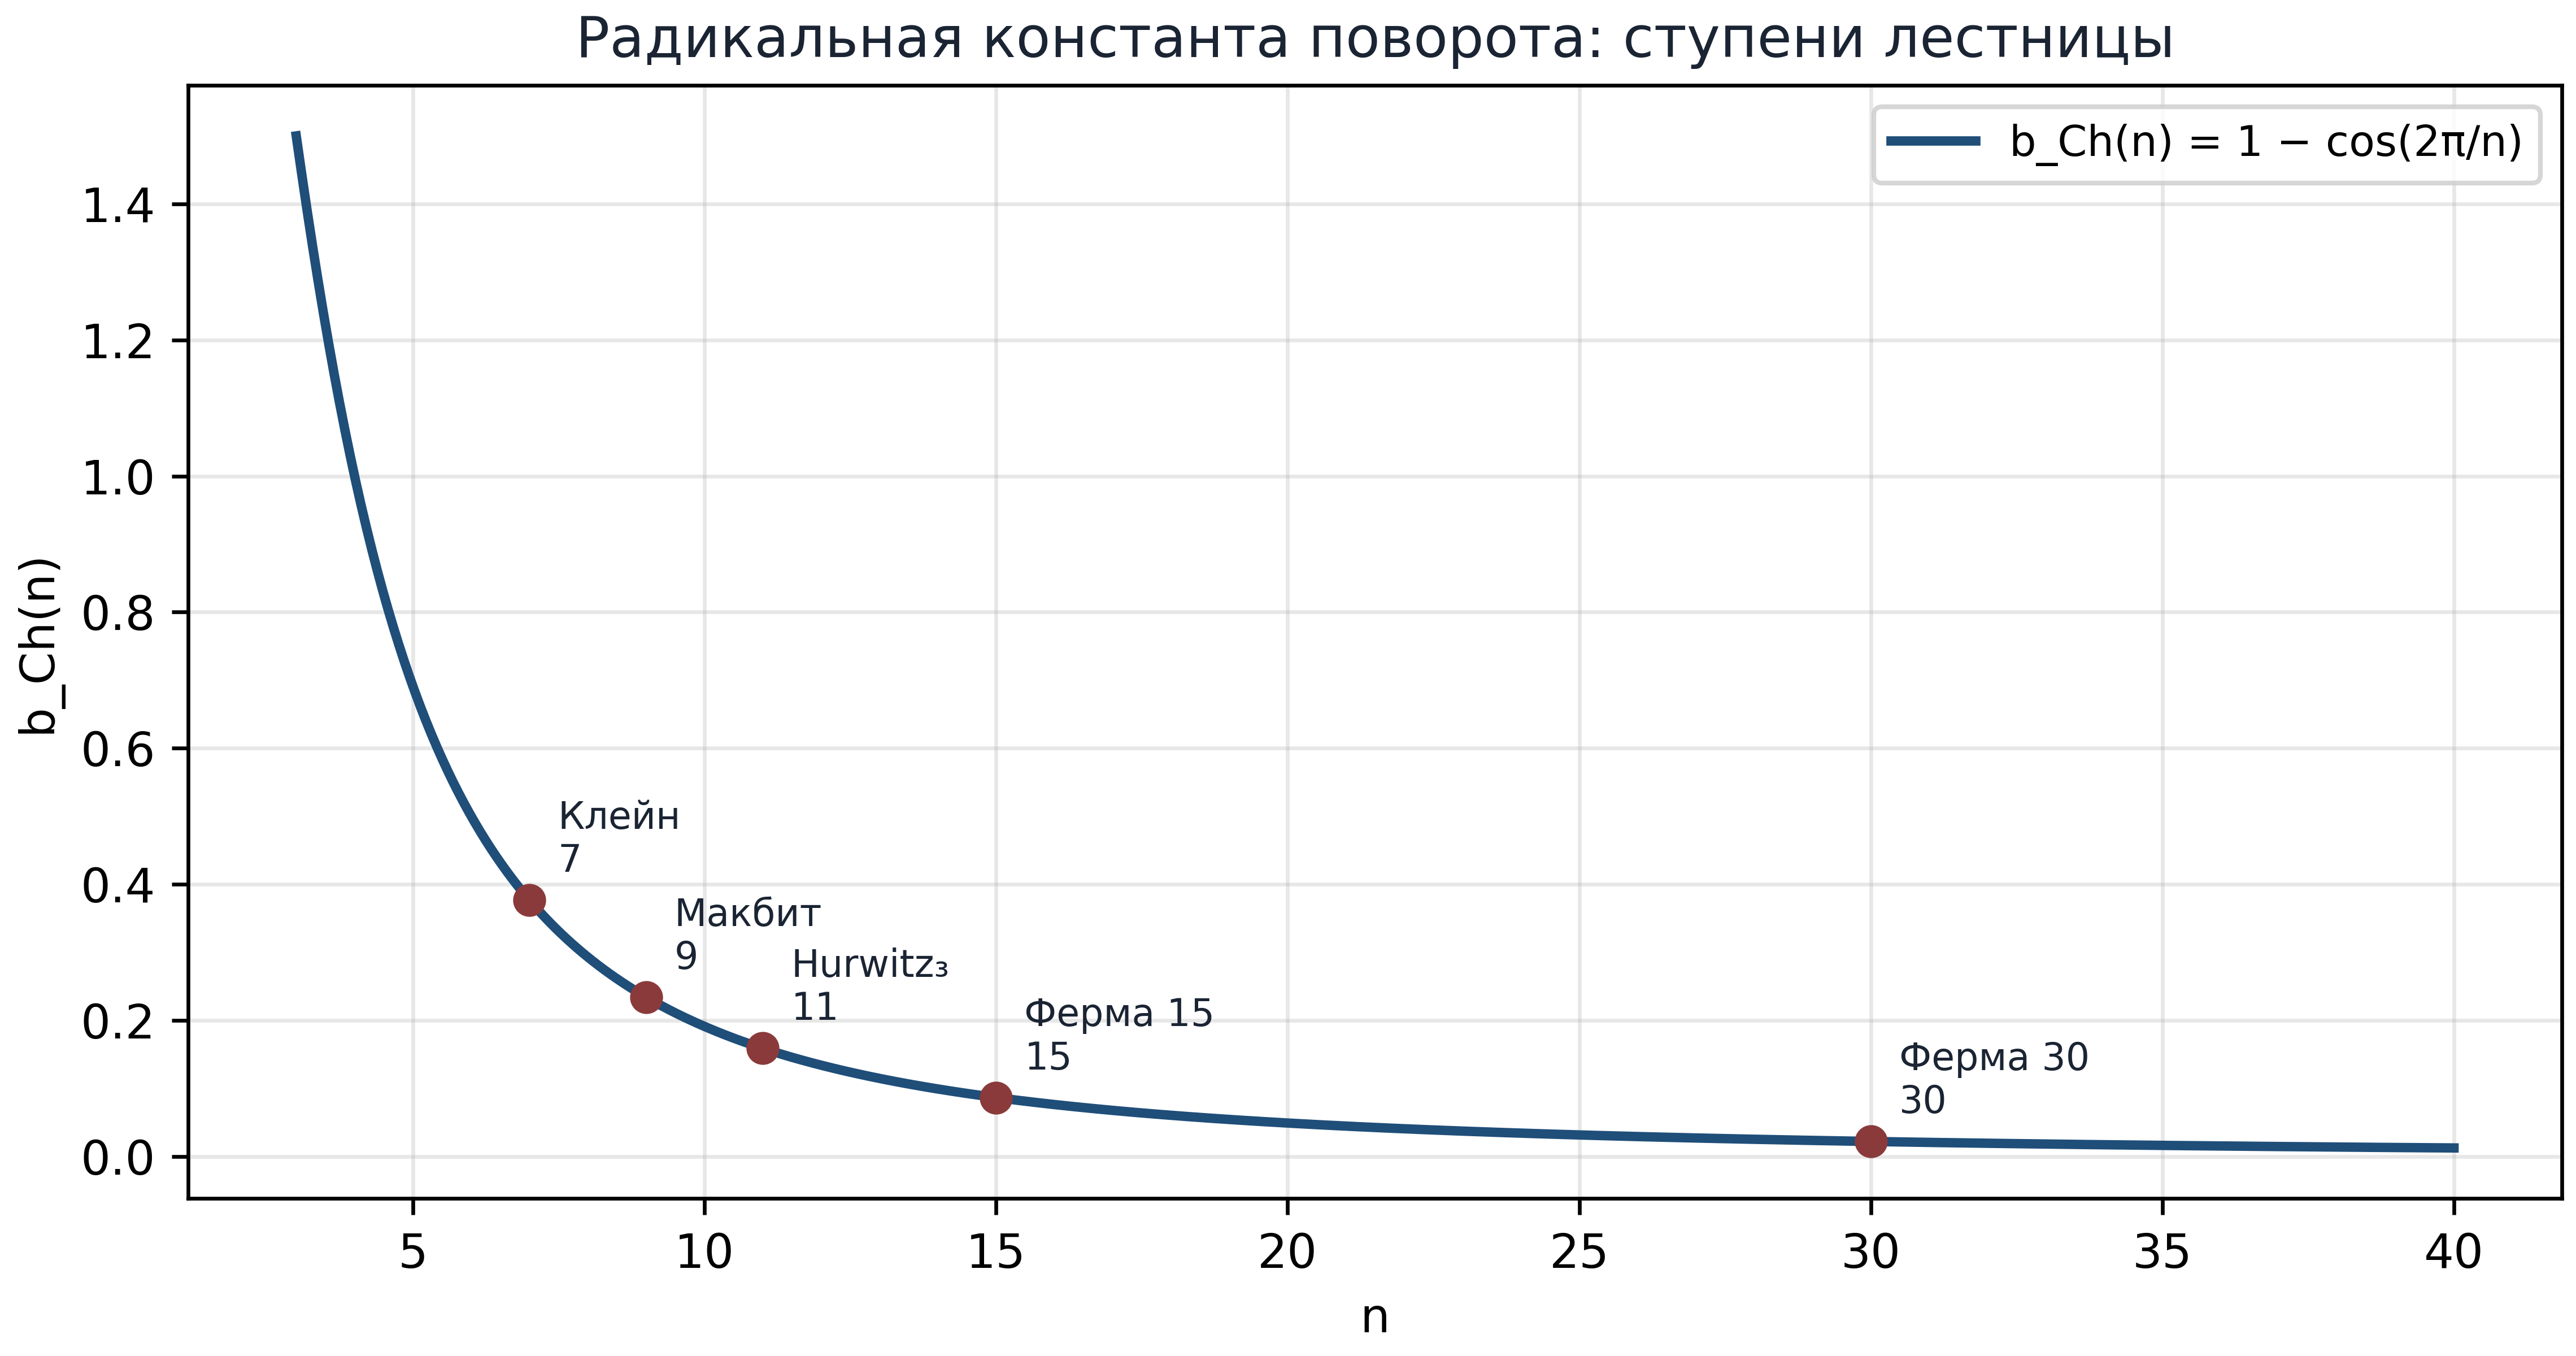
\includegraphics[width=0.82\textwidth]{figs/fig_bch.png}
\caption{Радикальная константа поворота $b_{Ch}(n)=1-\cos(2\pi/n)$
с отмеченными ступенями лестницы: Клейн ($n=7$), Макбит ($9$),
Hurwitz$_3$ ($11$), Ферма $15$ и $30$. На уровнях стенда константа
принимает точные радикальные значения
\eqref{eq:b15}--\eqref{eq:b30} (теорема~\ref{th:normalization},
пункт~4).}
\label{fig:bch}
\end{figure}

\begin{figure}[t]
\centering
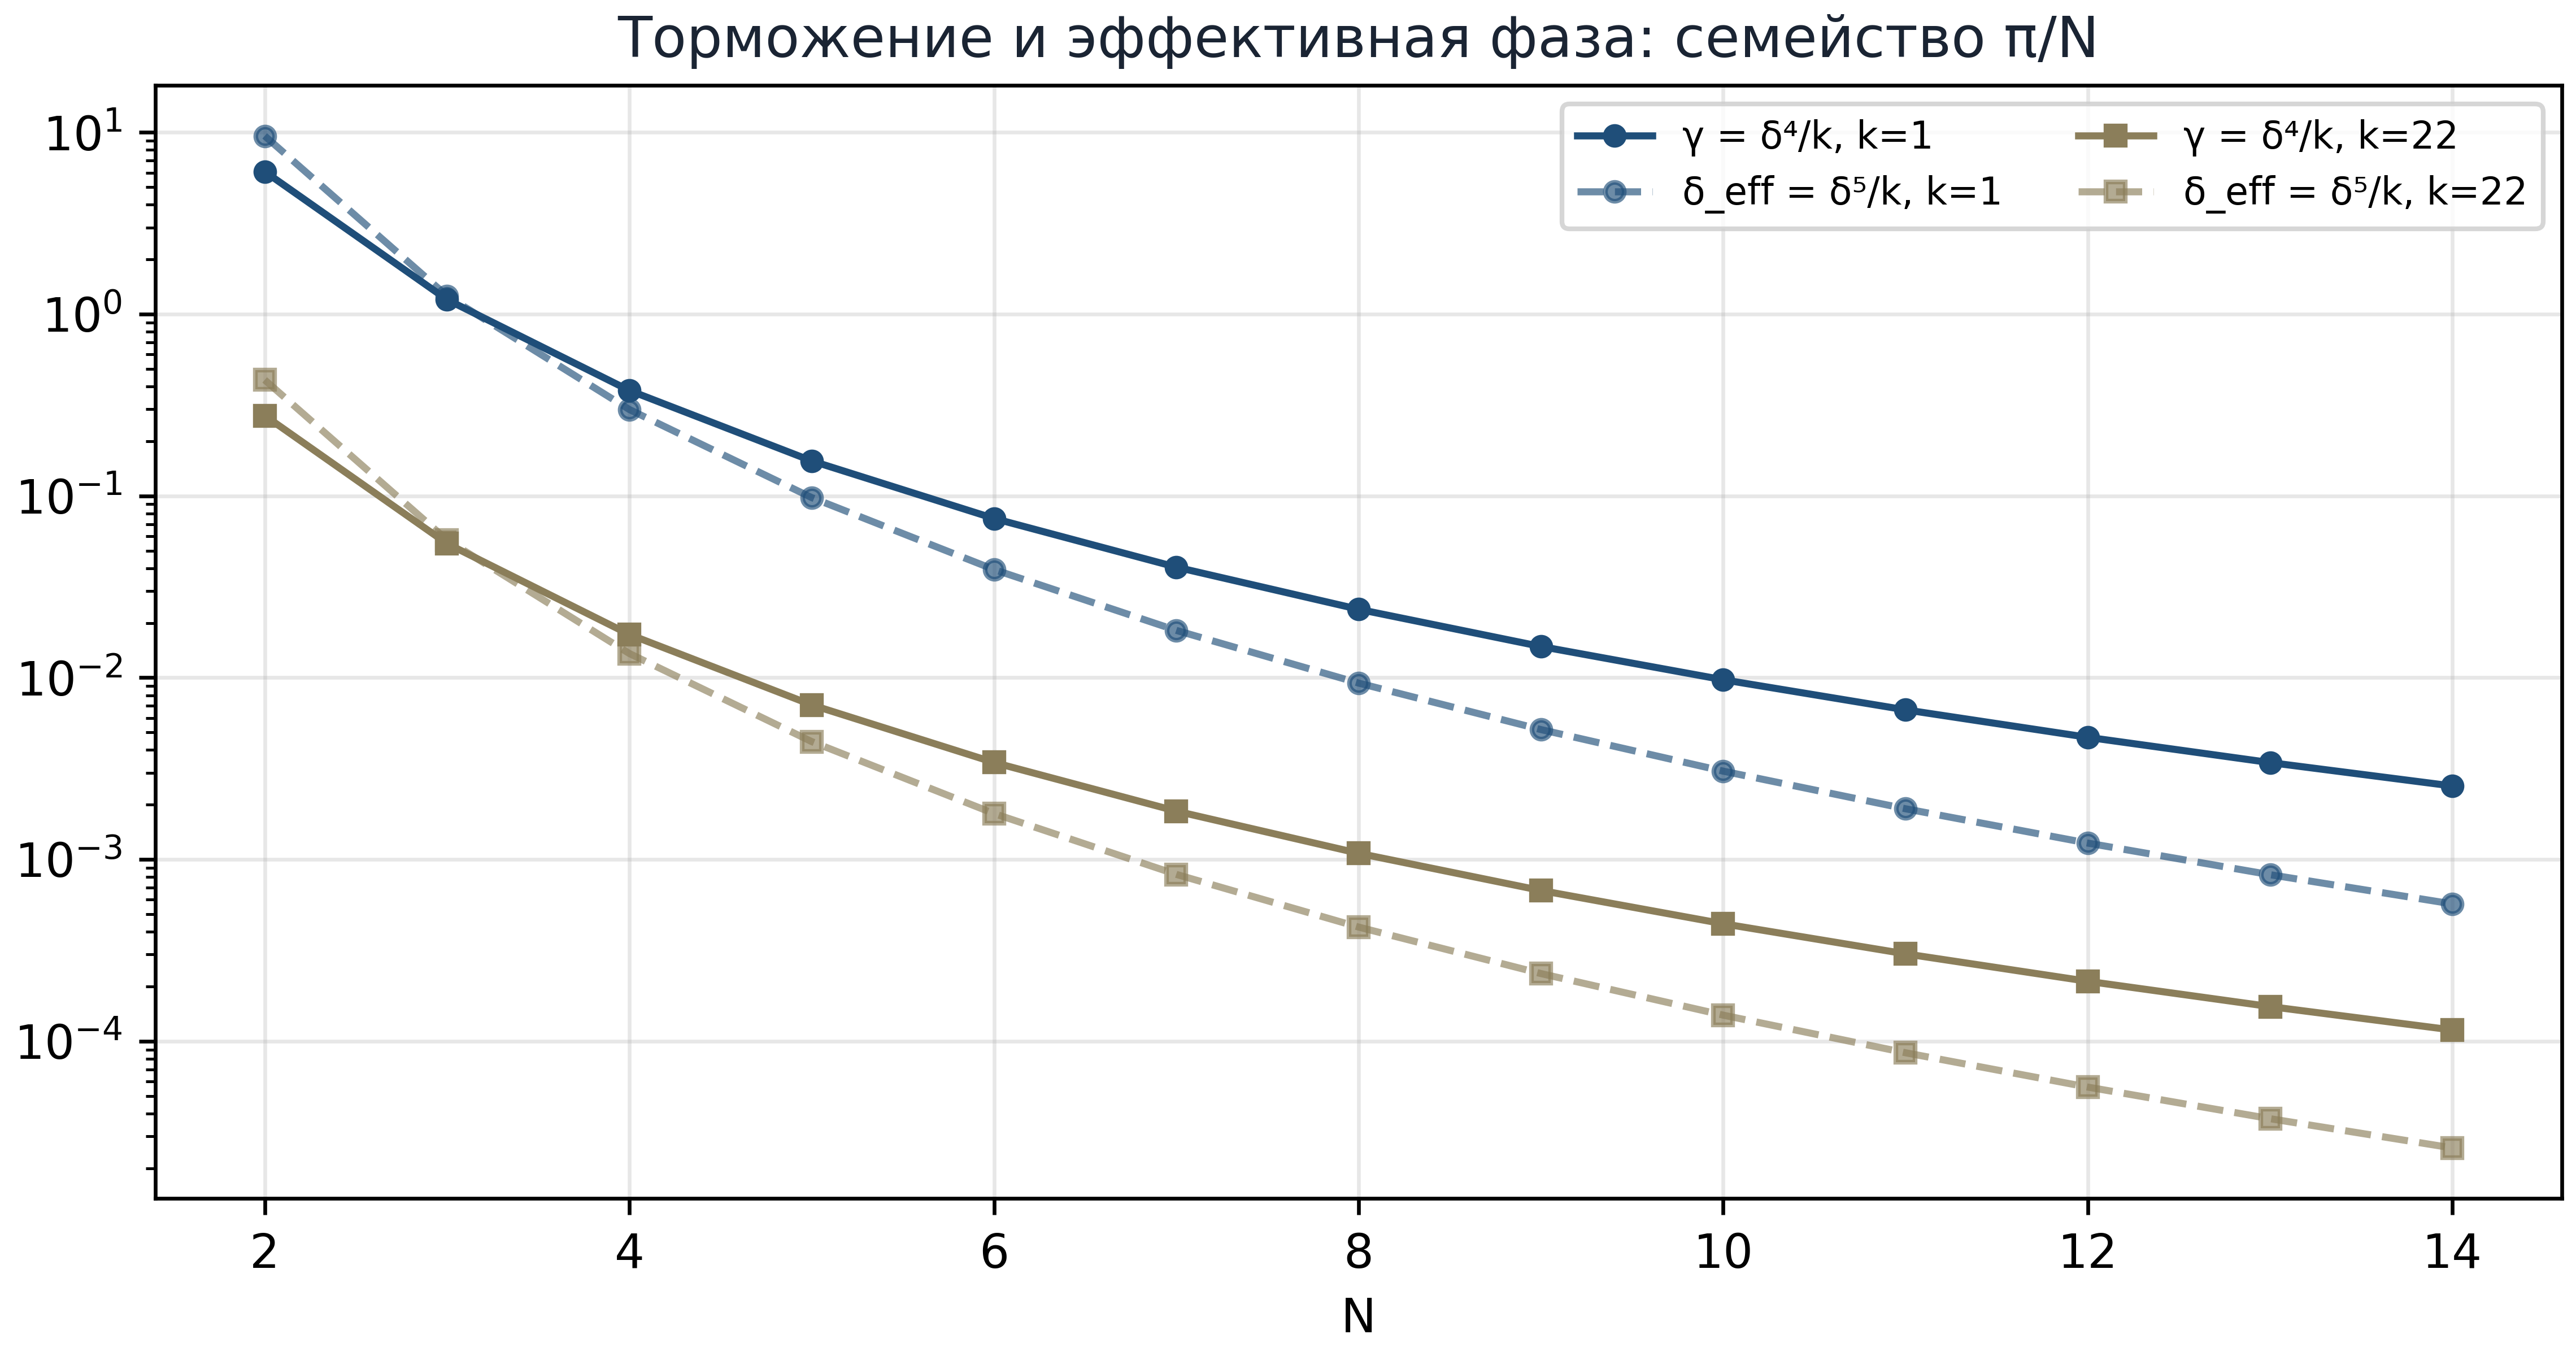
\includegraphics[width=0.82\textwidth]{figs/fig_torus.png}
\caption{Семейство торможений $\gamma=\delta^4/k$ и эффективных
фаз $\delta_{\mathrm{eff}}=\delta^5/k$ для $k\in\{1,22\}$ ---
два носителя на графике дают два семейства кривых; носитель $k=22$
подавляет поправку на два порядка. Данные соответствуют
таблице приложения~\ref{app:fulldata} и разделу~\ref{sec:torus}.}
\label{fig:torus}
\end{figure}

\begin{figure}[t]
\centering
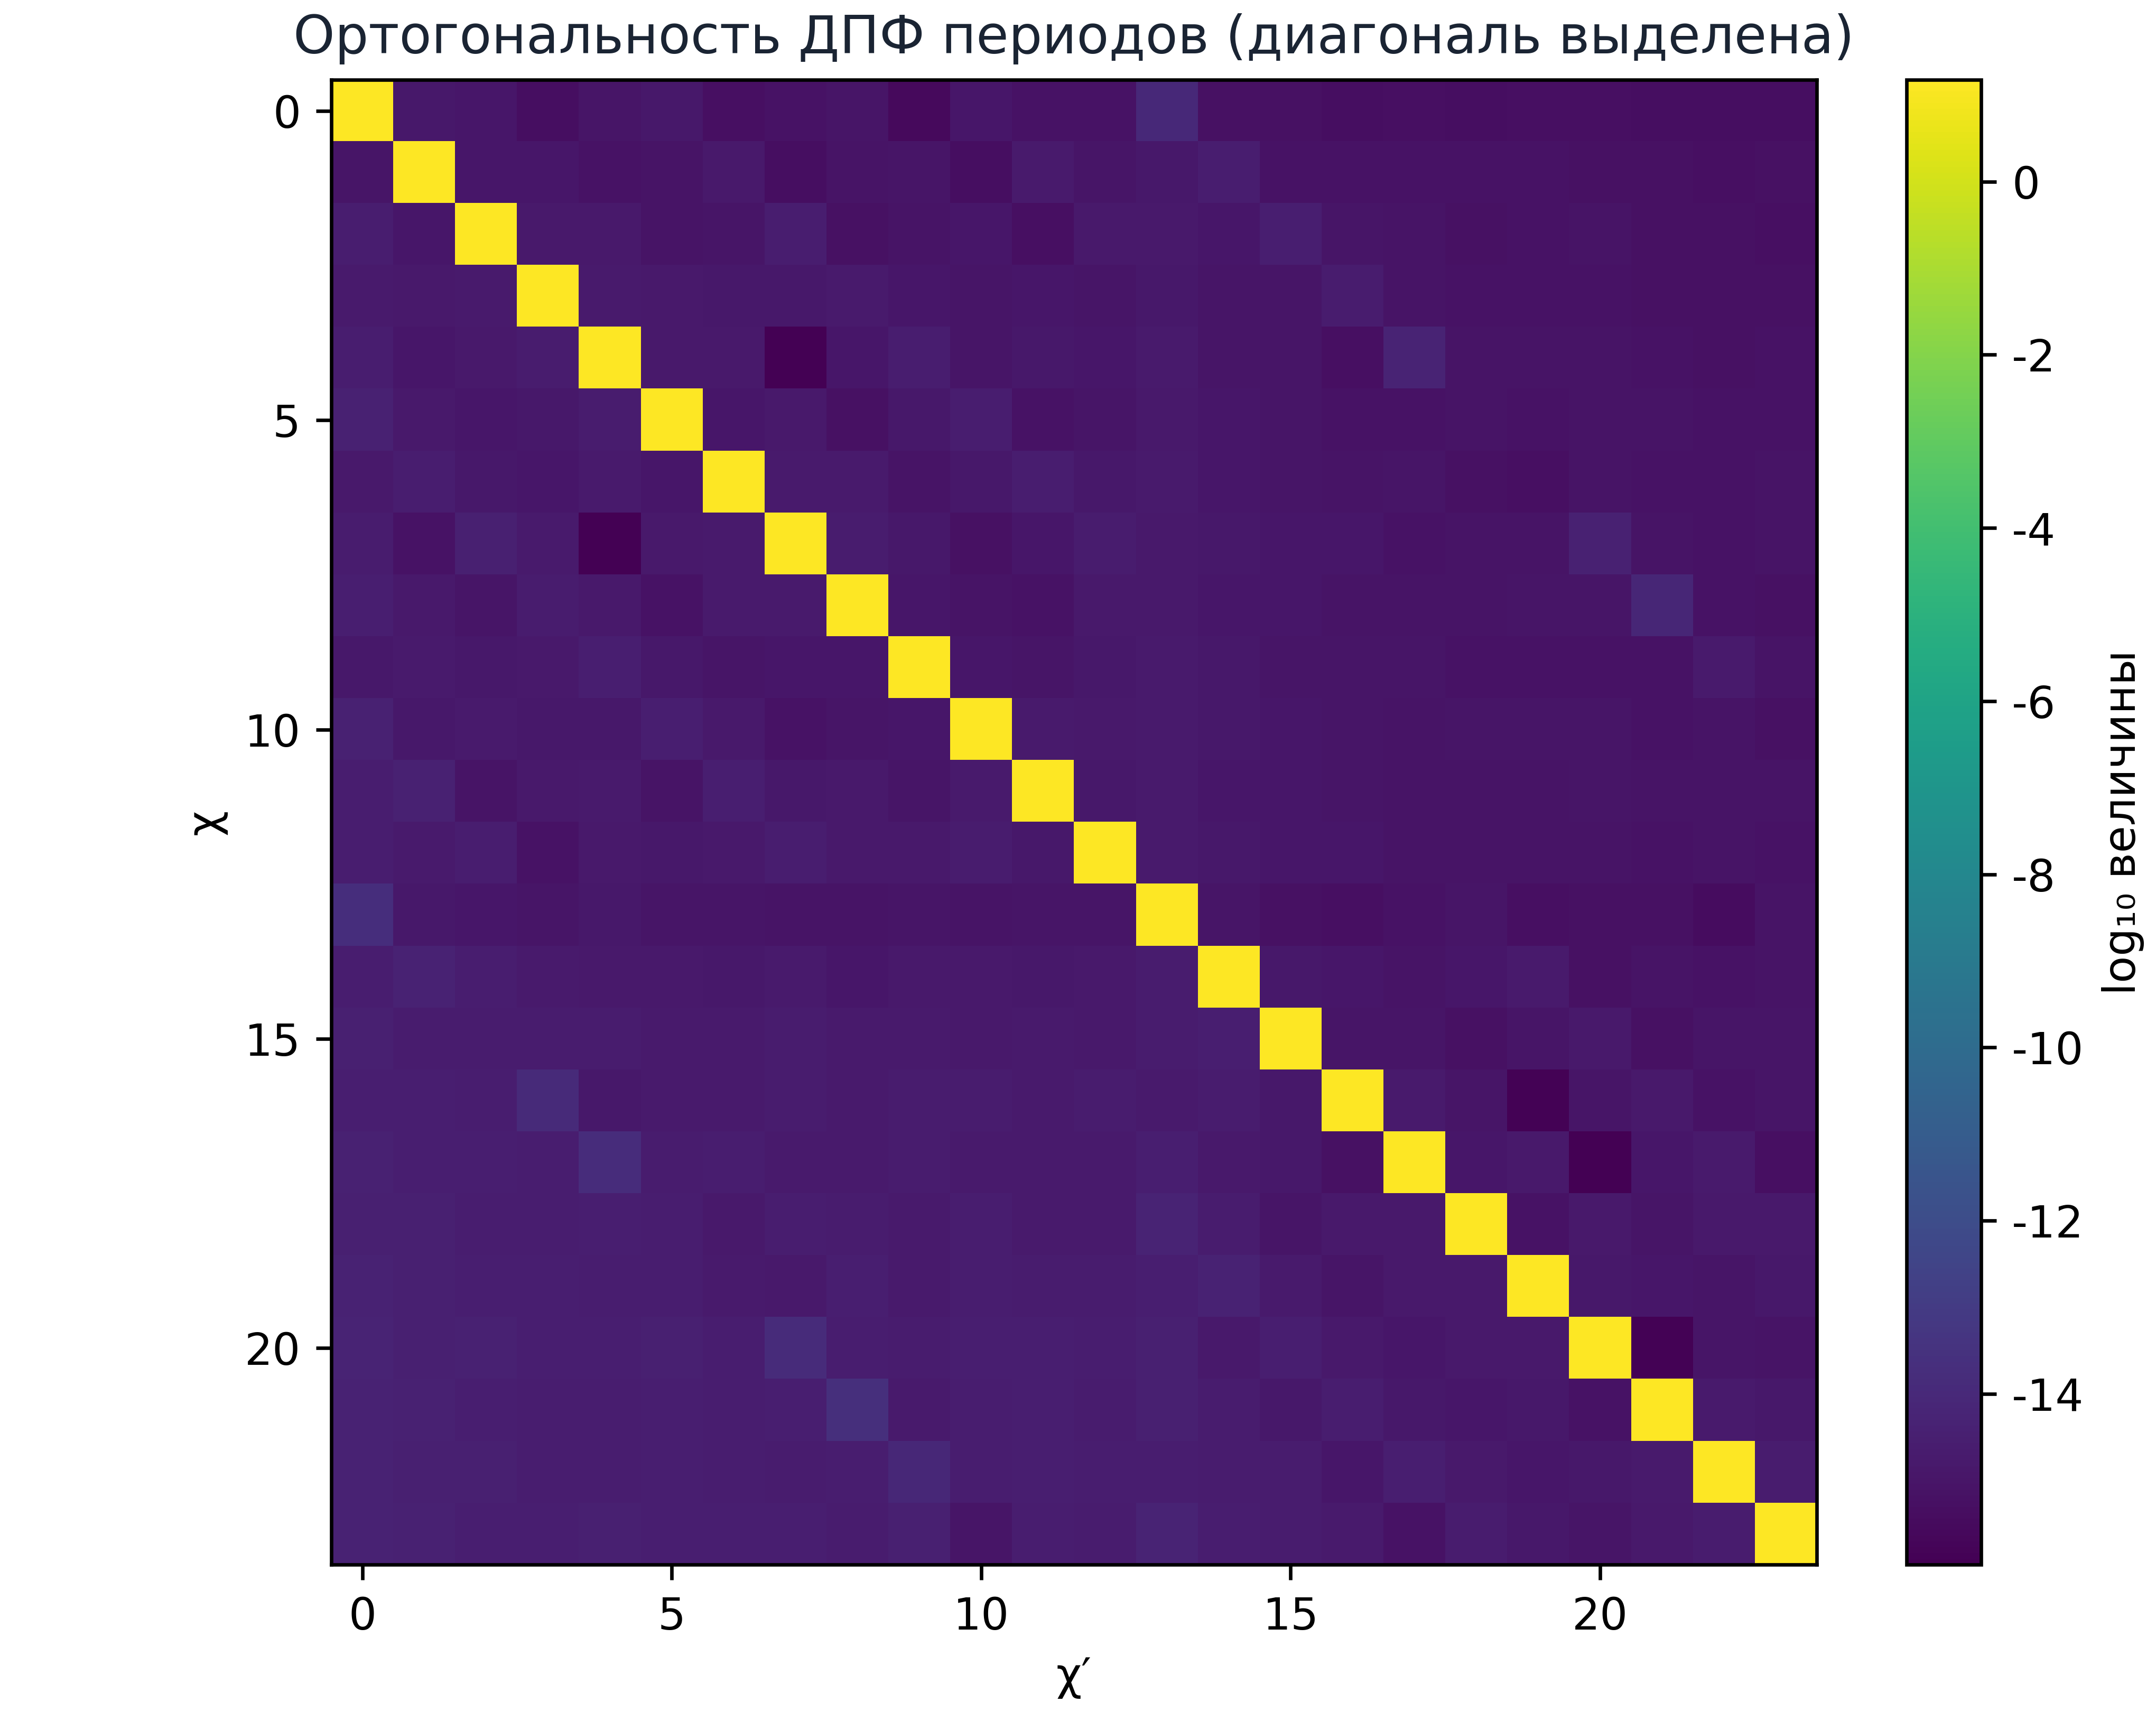
\includegraphics[width=0.78\textwidth]{figs/fig_dft.png}
\caption{Матрица величин $|\sum_{r,s}P_\chi\overline{P_{\chi'}}|$
(логарифмическая шкала): яркая диагональ ---
$|\Omega_\chi|^2$, внедиагональный фон на уровне $10^{-37}$
относительно диагонали --- численный портрет ортогональности ДПФ
(проверка V8). Ортогональность --- прямое следствие полноты
системы характеров группы $(\ZZ/N)^2$.}
\label{fig:dft}
\end{figure}

\section{Каталог формул}\label{sec:formulas}

Полный каталог формул программы с указанием номеров и мест
вывода --- справочная страница монографии.

\begin{center}
\small
\begin{longtable}{@{}p{3.2cm} p{8.2cm} p{2.6cm}@{}}
\toprule
Формула & Содержание & Вывод \\
\midrule
\endfirsthead
\toprule
Формула & Содержание & Вывод \\
\midrule
\endhead
\bottomrule
\endfoot
$\delta=\pi/N$ & спиновая фаза поворота порядка $N$ &
\eqref{eq:delta} \\
$\gamma=\delta^4/k$ & торможение по индексу носителя &
\eqref{eq:gamma} \\
$\delta_{\mathrm{eff}}=\delta^5/k$ & эффективная фаза &
\eqref{eq:deff} \\
$\Delta_{Ch}$ & объединённая формула поправок & \eqref{eq:deltaCh} \\
$b_{Ch}(n)$ & радикальная константа поворота & \eqref{eq:deltaCh} \\
$g=\tfrac{(N-1)(N-2)}2$ & род кривой Ферма & лемма
\ref{lem:genus} \\
$\chi(C_N^\circ)=-N^2$ & эйлерова характеристика проколотой кривой &
лемма \ref{lem:gridgraph} \\
$\rank K=3N-1$ & ядро замыкания циклов & лемма \ref{lem:capping} \\
$J=\begin{pmatrix}0&I\\-I&0\end{pmatrix}$ & симплектическая матрица
пересечений & лемма \ref{lem:sympl} \\
$\eta_{i,j}$ & базис голоморфных форм & лемма \ref{lem:forms} \\
$d=N/\gcd(N,a,b)$ & проводник характера & опр. \ref{def:conductor} \\
$h_d$ & перепись по Мёбиусу & \eqref{eq:mobius} \\
$P=\tfrac1N\zeta^{ra+sb}\Omega_{a,b}$ & замкнутая форма периода &
лемма \ref{lem:closedform} \\
$\Omega_{a,b}=\Bfun(a/N,b/N)$ & бета-значение & \eqref{eq:omegaab} \\
$\Ga(z)\Ga(1-z)=\pi/\sin\pi z$ & формула отражения &
\eqref{eq:reflection} \\
$\prod\Ga(z+k/m)=\dots$ & формула умножения Гаусса &
\eqref{eq:gauss} \\
$\Omega^{T}=\Omega$, $\im\Omega\succ0$ & соотношения Римана &
теорема \ref{th:riemann} \\
$\widehat P=P/\Omega_{a,b}$ & $\Ga$-нормировка & опр.
\ref{def:grossnorm} \\
$b_{Ch}(15)$, $b_{Ch}(30)$ & радикалы стенда &
\eqref{eq:b15}--\eqref{eq:b30} \\
$\Ind(\Lambda_d)$ & индекс блока проводника & опр. \ref{def:indices} \\
$\lambda_{m,n}=(2\pi)^2|m\tau-n|^2/(\im\tau)^2$ & спектр решётки &
теорема \ref{th:certG} \\
$\mathrm{vol}_h=(2\pi)^{32}\prod\Ga(k/N)^{-c_k}$ & объём в полной
$\Ga$-нормировке & теорема \ref{th:H2} \\
$t^*=\lcm(W/\gcd(a,W),H/\gcd(b,H))$ & время завершимости потока &
теорема \ref{th:E} \\
$2\varepsilon<1/Q^2$ & радиус единственности рационализации &
теорема \ref{th:F} \\
$Q_{\text{стенд}}=480$ & граница знаменателей стенда &
теорема \ref{th:H56} \\
\end{longtable}
\end{center}
